\chapter{Intermediate Representation (IR) Model}
\label{ch:ir_formalization}

\section{Introduction}
The analysis pipeline described in Chapter \ref{ch:analysis_pipeline}
is structured as a composition of typed transformations. Given a
source file $S$ belonging to a language $L \in \mathcal{L}$,
Tree-sitter produces a Concrete Syntax Tree (CST), which is then
transformed by the extraction function $\varepsilon$ (detailed in Chapter
\ref{ch:extraction}) into a forest of Module hierarchies:
$$\varepsilon : \mathcal{L} \times \mathcal{S}_{code} \to \vec{\mathcal{M}}$$
The goal of this chapter is to formally define the domain
$\mathcal{D}$ of the Intermediate Representation, i.e., the
set of all valid Module hierarchies $\vec{\mathcal{M}}$ that can be
produced by the extraction function. The IR is designed as a
\textit{conservative extension} \cite{aho_compilers_2007}
of the high-level syntactic constructs shared across languages: it
preserves the essential architectural semantics (types, functions,
fields, inheritance, modules) while abstracting away
language-specific syntactic details.

The subsequent phases of the pipeline, Name Resolution ($\rho$,
Chapter \ref{ch:name_resolution}) and Graph Construction ($\gamma$,
Chapter \ref{ch:graph_construction}), operate exclusively on
$\mathcal{D}$, which guarantees that their logic is completely
language-independent.

\section{The Type System}
To ensure language agnosticism, we define the type system as an
algebra of sum and product types \cite{pierce_types_2002}.

\subsection{Identifiers and Paths ($\pi$)}
Let $\mathcal{I}$ be the set of valid strings as identifiers. We
define the path domain $\Pi$ and the type \textbf{Qualified Name} ($\pi$)
as the set of finite non-empty sequences of identifiers:
$$\Pi = \mathcal{I}^+ = \{ \langle \iota_1, \iota_2, \dots, \iota_n \rangle \mid
\iota_j \in \mathcal{I}, n \geq 1 \}, \qquad \pi \in \Pi$$
This type uniquely maps namespaces, Java packages, Rust modules, and
resolved scopes in C++.

\subsection{Type References ($\tau$)}
A type reference $\tau$ in the IR models the lifecycle of symbol
discovery and resolution. To guarantee \textit{Type Safety} between
the extraction phases and the graph generation, we define $\tau$ as
an eight-state sum type:
\begin{align*}
  \tau ::=&\ \text{Prim}(\iota_p) \quad (\iota_p \in \mathcal{P}) \\
  &\mid \text{Unresolved}(\pi_{raw}) \\
  &\mid \text{ResolutionQuery}(\mathcal{Q}) \\
  &\mid \text{Resolved}(\pi_{abs}) \\
  &\mid \text{External}(\pi_{ext}) \\
  &\mid \text{Union}(\vec{\tau}) \\
  &\mid \text{EvaluatedAccess}(\tau_{path}, \tau_{type}) \\
  &\mid \text{Failed}(\pi_{raw})
\end{align*}
Where:
\begin{itemize}
  \item \textbf{Prim}: Represents fundamental primitive types
    ($\iota_p \in \mathcal{P}$). Since primitive keywords vary drastically
    across languages, the set $\mathcal{P}$ is not static but
    provided by a Data-Driven architectural \textit{Primitive
    Registry} populated at load time. Being defined at the language
    level, they do not require resolution.
  \item \textbf{Unresolved}: A raw text path extracted by the parser
    before any substitution.
  \item \textbf{ResolutionQuery($\mathcal{Q}$)}: Represents an
    algebraic expression composed of \texttt{Find}, \texttt{Extract},
    and \texttt{Call} operations. It is the partial product that
    defers resolution to Phase 2.
  \item \textbf{Resolved}: Represents a user-defined type (internal
    to the project) whose declaration or definition has been
    successfully localized and associated within the absolute
    namespace of the project. The path $\pi_{abs}$ is relative to the
    root of the module tree.
  \item \textbf{External}: Represents a type that is recognized and
    spatially localized, but belongs to a module or ecosystem outside
    the provided source code (e.g., standard libraries,
    \texttt{java.util.*}, external crates).
  \item \textbf{Union($\vec{\tau}$)}: Captures a disjunction of types
    (e.g., \texttt{Union[A, B]} in Python or \texttt{A | B} in
    TypeScript). It maintains a vector of references that must be
    individually processed.
  \item \textbf{EvaluatedAccess($\tau_{path}, \tau_{type}$)}: A
    wrapper that preserves both the originally queried path and the
    final structural type. This ensures that intermediate access
    chains generate corresponding dependency edges.
  \item \textbf{Failed($\pi_{raw}$)}: Indicates that the static
    resolution phase has failed. It keeps track of the target path to
    support fallback analysis and calculate statistical metrics on
    \textit{Recall} (coverage and confidence of the analyzer).
\end{itemize}

Figure \ref{fig:typeref_lifecycle} illustrates the complete state
machine of a type reference during the analysis pipeline. This
rigorous separation allows the type system to enforce that graph
generation occurs exclusively from \texttt{Resolved} or
\texttt{External} references.

\begin{figure}[htpb]
  \centering
  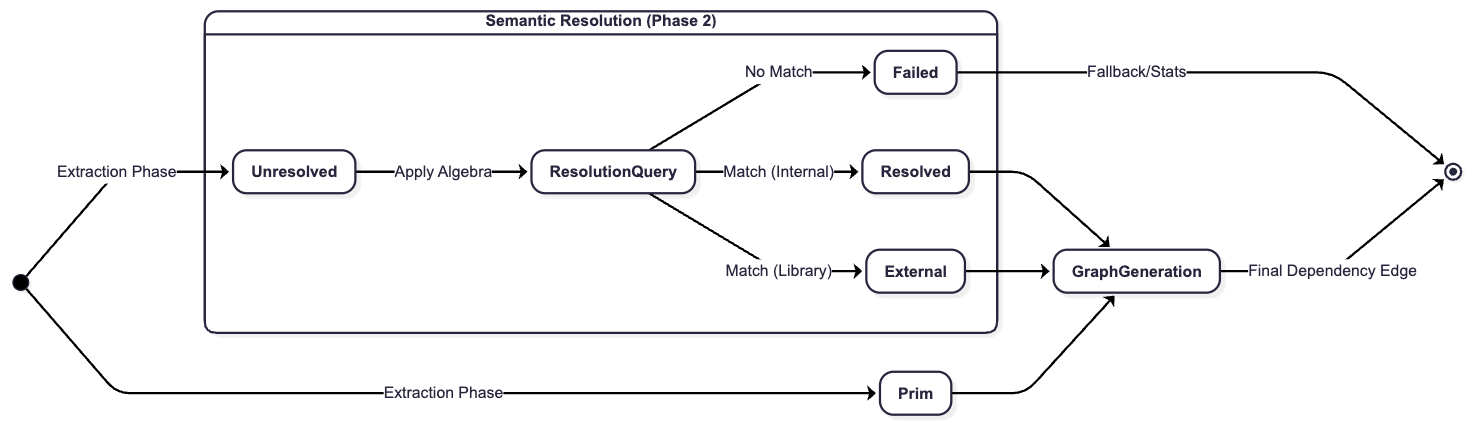
\includegraphics[width=\textwidth]{images/formal_ir/typeref_lifecycle.png}
  \caption{State machine diagram illustrating the lifecycle of a Type
  Reference ($\tau$) from syntactic extraction to semantic resolution.}
  \label{fig:typeref_lifecycle}
\end{figure}

\section{Modeling Structural Constructs}
Structured Types represent the core of the architectural analysis.
They are modeled as product types whose components define the state
and behavior of the entity.

\subsection{Members and Signatures}
We define the \textbf{Field} type ($f$), representing an attribute or
data field. A field is modeled as the tuple of an identifier
$\iota \in \mathcal{I}$, a type reference $\tau$, and a vector of
annotation type references:
$$f = \langle \iota, \tau, \vec{\tau}_{ann} \rangle$$

We define the \textbf{Parameter} type ($p$) for function parameters:
$$p = \langle \iota^?, \tau, \mathbb{B} \rangle$$ where the identifier
$\iota^?$ is optional (to support lambda functions and anonymous
parameters), $\tau$ is the declared type, and $\mathbb{B}$ indicates
whether the parameter is variadic.

To abstract the concept of a function's ``signature'' from the
component that implements it, we introduce the \textbf{Signature}
type ($\sigma$):
$$\sigma = \langle \vec{p}, \tau_{ret} \rangle$$
where $\vec{p}$ is the ordered parameter vector and $\tau_{ret}$ is
the return type reference.

Building on this, to model the hierarchical body of a function, we
introduce the \textbf{Block} construct ($\mathcal{B}$). A lexical
block (typically delimited by braces \texttt{\{\}}) isolates an
internal scope where local variables can be declared. Leveraging the
same structure as data fields ($f = \langle \iota, \tau, \dots \rangle$), local
variables are elegantly formalized as a vector of $f$. The block
tracks its behavioral dependencies and can recursively nest further
blocks (as in \texttt{if} or \texttt{while} statements):
$$\mathcal{B} = \langle \vec{f}_{local}, \vec{\tau}_{calls},
\vec{\tau}_{inst}, \vec{\tau}_{accesses}, \vec{\tau}_{casts},
\vec{\mathcal{B}}_{sub} \rangle$$
where $\vec{\tau}_{calls}$ represents the set of type references
whose functions are explicitly invoked within the block,
$\vec{\tau}_{inst}$ represents the structured types explicitly
instantiated (e.g., via \texttt{new}), $\vec{\tau}_{accesses}$
represents the direct read or write references to a component's
state, and $\vec{\tau}_{casts}$ captures explicit type casts (e.g.,
\texttt{as} conversions or C-like casts).

Finally, we define the universal \textbf{Function} type
($\mathcal{F}$) as a container that binds a qualified name to a
specific signature, an optional root block modeling its body, a
boolean flag for constructors, and a vector of annotations:
$$\mathcal{F} = \langle \pi, \sigma, \mathcal{B}^?,
\mathbb{B}_{ctor}, \vec{\tau}_{ann} \rangle$$

The architectural role of an $\mathcal{F}$ (whether it acts as a
Method or a Free Function) is not encoded in its type, but is
determined exclusively by the structural context in which it is
placed (within a structured type or a module).

Overloading is naturally handled within the Intermediate Representation
by the set of functions of an entity: a structured type or module can contain
multiple functions sharing the same base identifier $\iota$ (or qualified name
$\pi$) but distinguished by distinct signatures $\sigma$. When the IR is
projected into the architectural dependency graph (Chapter
\ref{ch:graph_construction}),
overloaded variants sharing the same qualified path $\pi$ coalesce into a
single graph vertex, prioritizing component-level coupling and architectural
dependencies over fine-grained signature differentiation.

\subsection{Structured Types ($\mathcal{S}$)}
Let $\text{Kind} = \{ \text{Class, Struct, Interface, Trait, Enum,
EnumVariant} \}$ be the domain of structured type categories. A
structured type is defined by the tuple:
$$\mathcal{S} = \langle \pi, k \in \text{Kind}, \vec{f},
\vec{\mathcal{F}}, \vec{\tau}_{sup}, \vec{\mathcal{S}}_{nest},
\vec{\tau}_{ann}, \vec{\delta}_{imp} \rangle$$
where:
\begin{itemize}
  \item $\pi$: the qualified name identifying the entity within the system.
  \item $k$: the structural category (defined in $\text{Kind}$) that
    preserves the original semantics of the construct.
  \item $\vec{f}$: the vector of fields that compose the state of the entity.
  \item $\vec{\mathcal{F}}$: the vector of functions (assuming the role
    of methods) that define the behavior of the entity.
  \item $\vec{\tau}_{sup}$: the vector of references to super-types,
    modeling inheritance or trait/interface implementation relationships.
  \item $\vec{\mathcal{S}}_{nest}$: the vector of nested types.
  \item $\vec{\tau}_{ann}$: the vector of annotation, attribute, or
    decorator type references applied to the entity.
  \item $\vec{\delta}_{imp}$: the vector of import declarations
    visible within the scope of the structured type (see the
    definition of $\delta_{imp}$ in Section \ref{sec:module_def}).
\end{itemize}

\begin{lstlisting}[language=Java,caption={An example of a structured type in Java}]
@Entity
public class Car extends Vehicle implements Serializable {
    private Engine engine;
    private int speed;

    public void accelerate(int amount) { ... }
}
\end{lstlisting}

This is modeled in the IR as:
$\mathcal{S} = \langle \langle\texttt{Car}\rangle, \text{Class},
[\texttt{engine}: \tau_{\texttt{Engine}},\ \texttt{speed}: \tau_{\texttt{int}}],
[\texttt{accelerate}],
[\tau_{\texttt{Vehicle}},\ \tau_{\texttt{Serializable}}],
[\ ],
[\tau_{\texttt{Entity}}],
[\ ] \rangle$

\subsection{Type Alias ($\mathcal{A}$)}
A \textbf{Type Alias} allows defining a new name for an existing
type. It is modeled as the tuple:
$$\mathcal{A} = \langle \pi, \tau_{target} \rangle$$
where $\tau_{target}$ is the reference to the original type. During
graph construction, type aliases are maintained as independent nodes
to accurately track the semantic use of domains.

For example, the Rust declaration \texttt{type NodeId = usize;} is
modeled as $\mathcal{A} = \langle \langle\texttt{NodeId}\rangle,
\tau_{\texttt{usize}} \rangle$, and the C++ declaration
\texttt{using StringList = std::vector<std::string>;} as
$\mathcal{A} = \langle \langle\texttt{StringList}\rangle,
\tau_{\texttt{std::vector<std::string>}} \rangle$.

\subsection{Implementation Extensions ($\mathcal{X}$)}
To support languages that decouple the schema definition of a structured
type from the definition of its behavior and trait implementations (most
notably Rust via detached \texttt{impl} blocks), during extraction we
introduce the temporary construct \textbf{ImplBlock} or
\textbf{Implementation Extension}:
$$\mathcal{X} = \langle \pi, \tau_{target}, \tau_{trait}^?,
\vec{\mathcal{F}}, \vec{\mathcal{S}}_{nest}, \vec{\mathcal{A}} \rangle$$
where $\pi$ is the name of the extension (typically derived from the
target type), $\tau_{target}$ is the type to which the implementation
applies, $\tau_{trait}^?$ is an optional reference to the implemented
trait or interface, and the other fields represent functions, nested
types, and aliases associated with the extension.

For example, the following Rust code:
\begin{verbatim}
impl Display for Car {
    fn fmt(&self, f: &mut Formatter) -> Result { ... }
}
\end{verbatim}
is modeled as $\mathcal{X} = \langle \langle\texttt{Car}\rangle,
\tau_{\texttt{Car}}, \tau_{\texttt{Display}},
[\texttt{fmt}], [\ ], [\ ] \rangle$.

As detailed in Chapter \ref{ch:name_resolution}, implementation
extensions act as ``syntactic sugar'': their methods, nested types,
and traits are \textit{flattened} into the target structured type's
scope, effectively disappearing from the final architectural model.

\section{Component Architecture}
The entire software system is represented as a hierarchy of
\textbf{Module} instances ($\mathcal{M}$). A module recursively
aggregates structured types, functions, sub-modules, type aliases,
free variables, and implementation extensions. This hierarchical
structure constitutes the domain $\mathcal{D}$ of the
Intermediate Representation.

\subsection{Component ($\mathcal{C}$)}
We define a \textbf{Component} ($\mathcal{C}$) as the disjoint union
(sum type) of the definitive structural constructs of the system.
Each component represents the logical unit that can appear as a
vertex in the dependency graph:
\begin{align*}
  \mathcal{C} ::=&\ \text{Mod}(\mathcal{M}) \\
  &\mid \text{StructuredType}(\mathcal{S}) \\
  &\mid \text{TypeAlias}(\mathcal{A}) \\
  &\mid \text{Function}(\mathcal{F}) \\
  &\mid \text{Field}(\pi, \tau) \\
  &\mid \text{Primitive}(str) \\
  &\mid \text{External}(\pi)
\end{align*}

\subsection{Module ($\mathcal{M}$)}
\label{sec:module_def}
The entire program structure is captured by the \textbf{Module} type
($\mathcal{M}$), defined recursively to reflect the hierarchy of the
file system or namespaces:
$$\mathcal{M} = \langle \pi, str_{lang}^?, str_{path}^?,
\vec{\delta}_{imp}, \vec{\mathcal{M}}_{nest}, \vec{\mathcal{S}},
\vec{\mathcal{A}}, \vec{\mathcal{F}}, \vec{f}_{free},
\vec{\mathcal{X}} \rangle$$
where:
\begin{itemize}
  \item $\pi$: the qualified name of the module.
  \item $str_{lang}^?$: an optional string indicating the source
    language (e.g., \texttt{"rust"}, \texttt{"java"}).
  \item $str_{path}^?$: an optional string representing the file
    system path of the source file.
  \item $\vec{\delta}_{imp}$: the vector of \textbf{Import}
    declarations. Each import $\delta_{imp}$ is a product type:
    $$\delta_{imp} = \langle \pi_{path}, \iota_{alias}^?,
    \mathbb{B}_{wildcard} \rangle$$
    where $\pi_{path}$ is the import path,
    $\iota_{alias}^?$ is an optional alias name (e.g.,
    \texttt{import numpy as np} $\to$ $\iota_{alias} = \texttt{np}$),
    and $\mathbb{B}_{wildcard}$ is a boolean flag indicating whether
    the import is a wildcard inclusion (e.g., \texttt{from module
    import *}).
  \item $\vec{\mathcal{M}}_{nest}$: the vector of nested sub-modules.
  \item $\vec{\mathcal{S}}$: the vector of structured types defined
    in this module.
  \item $\vec{\mathcal{A}}$: the vector of type aliases.
  \item $\vec{\mathcal{F}}$: the vector of free functions (not
    belonging to any structured type).
  \item $\vec{f}_{free}$: the vector of free variables (global
    constants, static items).
  \item $\vec{\mathcal{X}}$: the vector of implementation extensions
    (to be flattened during name resolution).
\end{itemize}

A complete overview of the entities described so far, their
composition, and their semantic references is illustrated in Figure
\ref{fig:ir_model} via a UML class diagram.

\begin{figure}[htpb]
  \centering
  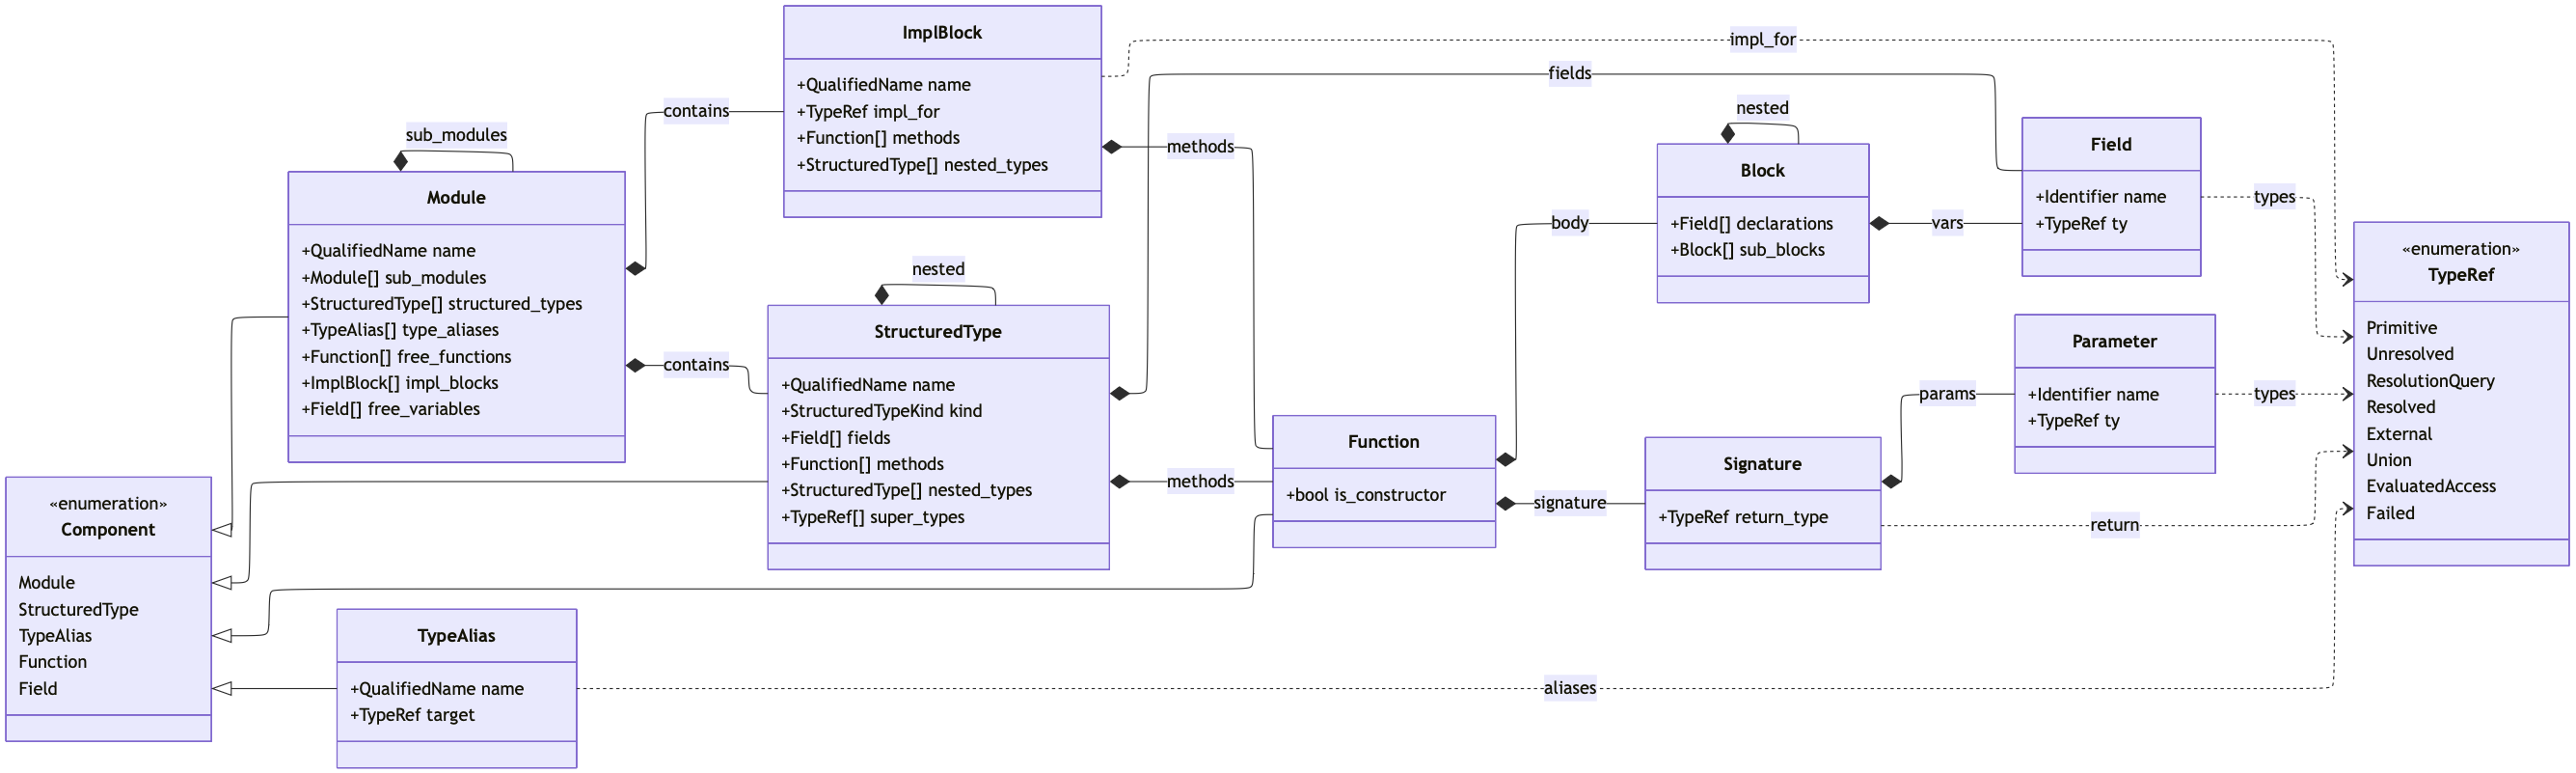
\includegraphics[width=\textwidth]{images/formal_ir/IR_model.png}
  \caption{UML class diagram representing the complete Intermediate
    Representation (IR) domain model, highlighting hierarchical
  composition and semantic references via \texttt{TypeRef}.}
  \label{fig:ir_model}
\end{figure}

\section{Analyzer Configuration ($\mathcal{K}$)}
\label{sec:analyzer_config}

A fundamental challenge in building a language-agnostic analyzer is
reconciling the semantic differences between languages without
introducing language-specific code branches. The approach adopted in
this work draws from the concept of \textbf{Language Product Lines}
\cite{vacchi_neverlang_2015}: rather than treating each
language as a monolithic entity, the analyzer decomposes languages
into a set of orthogonal \textbf{language features}. Each feature
represents a specific semantic capability (e.g., ``supports implicit
  self parameter'', ``uses transitive imports'', ``allows detached
implementation blocks'') that may or may not be present in any given
language. The analyzer's behavior is then parameterized by these
features, selecting the appropriate processing strategies at each
pipeline phase.

By modeling semantic capabilities as orthogonal configuration flags,
the analyzer decouples the core analysis logic from language-specific
syntactic and semantic details. Rather than implementing $M$ independent,
hard-coded analysis pipelines, supporting a new language becomes a declarative
task: identifying which semantic features the language exhibits and specifying
its configuration profile.

Formally, the analyzer configuration is modeled as a product type:
\begin{align*}
  \mathcal{K} = \langle&\ \text{ModuleConfig}, \\
  &\ \text{TransitiveImports}, \\
  &\ \text{SupportImplBlocks}, \\
  &\ \text{ForwardDeclarations}, \\
  &\ \text{SelfKeyword}, \\
  &\ \text{SelfTypeKeyword}, \\
  &\ \text{ImplicitFirstParamAsSelf}, \\
  &\ \text{ExtractDynamicFields}, \\
  &\ \text{DerefCoercionTargetName} \rangle
\end{align*}

This feature-based configuration model is the mechanism that makes
the resolution engine and graph construction phases truly
language-agnostic: they do not contain conditional branches on the
source language, but instead query the configuration flags to
determine the appropriate behavior.

The parameters are organized into three orthogonal dimensions:
module topology, declaration linking, and instance semantics.

\subsection{Module Organization Strategies}

The sub-configuration \textbf{ModuleConfig} models how source files
and directories are grouped into hierarchical module namespaces:
\begin{align*}
  \text{ModuleConfig} = \langle&\ \text{FileBased}, \\
  &\ \text{DirectoryBased}, \\
  &\ \text{PackageDeclBased}, \\
  &\ \text{NamespaceBased}, \\
  &\ \text{InlineModBased} \rangle
\end{align*}
Each boolean flag controls whether a specific grouping mechanism is active during extraction:
\begin{itemize}
  \item \textbf{File-Level Package Declarations (\texttt{PackageDeclBased})}: In languages such as Java, the compilation unit declares its enclosing namespace through a single statement at the top of the file (e.g., \texttt{package com.example.service;}). This statement assigns the entire file to the designated logical package without wrapping declarations in syntactic braces.
  \item \textbf{Filesystem-Inferred Hierarchies (\texttt{FileBased}, \texttt{DirectoryBased})}: Languages like Python and Rust infer module namespaces directly from the filesystem layout. Directories represent parent packages or modules, while individual source files correspond to leaf modules.
  \item \textbf{Open Namespace Blocks (\texttt{NamespaceBased})}: In C++, namespaces are explicit structural containers delimited by braces (e.g., \texttt{namespace core \{ ... \}}). Crucially, C++ namespaces are open and reopenable across distinct files and header units, bearing no intrinsic relationship to the directory layout.
  \item \textbf{Encapsulated Inline Modules (\texttt{InlineModBased})}: In Rust, the module system exhibits a dual nature. The keyword \texttt{mod} can appear as a file-level declaration without a body (\texttt{mod foo;}), which delegates to an external file or directory, or as an inline structural block (\texttt{mod foo \{ ... \}}). Unlike C++ namespaces, Rust inline modules are closed and non-reopenable scopes that nest within the enclosing filesystem module.
  \item \textbf{Absence of Modularization (Flat Root Module)}: The C language features neither package statements nor namespace containers. When all configuration flags evaluate to false, all extracted components are collected into a single, flat root module, matching the global symbol model of the C linker.
\end{itemize}

Table \ref{tab:lang_config_modules} summarizes these strategies across the supported languages.

\begin{table}[htbp]
  \centering
  \begin{tabular}{|l|c|c|c|c|c|}
    \hline
    \textbf{Language} & \textbf{FileBased} & \textbf{DirBased} &
    \textbf{PkgDecl} & \textbf{Namespace} & \textbf{InlineMod} \\ \hline
    \textbf{Java}     & False & False & True  & False & False \\ \hline
    \textbf{Rust}     & True  & True  & False & False & True  \\ \hline
    \textbf{Python}   & True  & True  & False & False & False \\ \hline
    \textbf{C++}      & False & False & False & True  & False \\ \hline
    \textbf{C}        & False & False & False & False & False \\ \hline
  \end{tabular}
  \caption{Module organization strategies across supported languages.}
  \label{tab:lang_config_modules}
\end{table}

\subsection{Declaration Linking and Visibility}

Languages differ fundamentally in how definitions are exposed across
boundaries and linked across compilation units:

\paragraph{Transitive Imports (\texttt{TransitiveImports})} In languages
such as Python, packages idiomatically re-export members of sub-modules
through \texttt{\_\_init\_\_.py} files, allowing consumers to access them
transitively. Conversely, in Java and Rust, imports are file-local by
default and require explicit re-export declarations (e.g., \texttt{pub use}).

\paragraph{Detached Implementation Blocks (\texttt{SupportImplBlocks})}
Languages like Rust separate the declaration of data structures
(\texttt{struct}, \texttt{enum}) from their behavior and trait implementations
(\texttt{impl} blocks), allowing multiple detached blocks to extend the same
type across different modules or files. This flag activates the extraction
of implementation extensions $\mathcal{X}$, which are later flattened into
the target structured type during resolution.

\paragraph{Forward Declarations (\texttt{ForwardDeclarations})}
The compilation model of languages such as C and C++ separates declarations
in header files (\texttt{.h}/\texttt{.hpp}) from definitions in source files
(\texttt{.c}/\texttt{.cpp}), admitting forward declarations of types and
functions across compilation units. In C++, member functions can be declared
inside a class body and defined out-of-line in separate translation units
using qualified identifiers (e.g., \texttt{ClassName::method}). Enabling this
flag activates an out-of-line method linking step that pairs detached method
implementations with their parent class declarations. This treats forward
declarations and out-of-line definitions as orthogonal to Rust-style
implementation blocks.

Table \ref{tab:lang_config_decl} summarizes the declaration and
linking profiles.

\begin{table}[htbp]
  \centering
  \begin{tabular}{|l|c|c|c|}
    \hline
    \textbf{Language} & \textbf{TransitiveImports} &
    \textbf{SupportImplBlocks} & \textbf{ForwardDeclarations} \\ \hline
    \textbf{Java}     & False & False & False \\ \hline
    \textbf{Rust}     & False & True  & False \\ \hline
    \textbf{Python}   & True  & False & False \\ \hline
    \textbf{C++}      & False & False & True  \\ \hline
    \textbf{C}        & False & False & True  \\ \hline
  \end{tabular}
  \caption{Declaration linking and visibility configuration profiles.}
  \label{tab:lang_config_decl}
\end{table}

\subsection{Instance Semantics and Receiver Resolution}

Resolving member accesses and invocations requires understanding how an
instance is referenced and how its members are declared within local scopes:

\paragraph{Receiver Binding (\texttt{SelfKeyword},
\texttt{ImplicitFirstParamAsSelf})}
In Java and C++, \texttt{this} is a language-level keyword providing an
implicit reference to the calling instance. In Rust, instance methods
explicitly declare \texttt{self} as their first parameter. In Python,
\texttt{self} is not a keyword, but a naming convention; Python instance
methods implicitly bind the calling instance to their first formal parameter
(\texttt{ImplicitFirstParamAsSelf} = \text{True}).

\paragraph{Dynamic Attribute Discovery (\texttt{ExtractDynamicFields})}
Unlike statically typed languages where fields are declared explicitly in the
type body, dynamic languages like Python frequently introduce instance fields
dynamically within constructor bodies via assignments of the form
\texttt{self.field = value}. Enabling this flag instructs the extractor to
inspect constructor ASTs and harvest these dynamic attributes.

\paragraph{Type Self-Reference and Deref Coercion
(\texttt{SelfTypeKeyword}, \texttt{DerefCoercionTargetName})}
Rust introduces the \texttt{Self} keyword to reference the implementing type
within an \texttt{impl} block. Furthermore, Rust's \texttt{Deref} trait
mechanism enables smart pointers to implicitly delegate method lookups to an
inner target type (\texttt{DerefCoercionTargetName} = \texttt{"Target"}),
a pattern traversed by the resolution engine during scope climbing.

Table \ref{tab:lang_config_inst} outlines the instance semantics and
receiver resolution features.

\begin{table}[htbp]
  \centering
  \small
  \begin{tabular}{|l|c|c|c|c|c|}
    \hline
    \textbf{Language} & \textbf{SelfKeyword} & \textbf{ImplicitSelf}
    & \textbf{DynamicFields} & \textbf{SelfType} &
    \textbf{DerefTarget} \\ \hline
    \textbf{Java}     & \texttt{this}        & False
    & False                  & ---               & ---
    \\ \hline
    \textbf{Rust}     & \texttt{self}        & False
    & False                  & \texttt{Self}     & \texttt{Target}
    \\ \hline
    \textbf{Python}   & ---                  & True
    & True                   & ---               & ---
    \\ \hline
    \textbf{C++}      & \texttt{this}        & False
    & False                  & ---               & ---
    \\ \hline
    \textbf{C}        & ---                  & False
    & False                  & ---               & ---
    \\ \hline
  \end{tabular}
  \caption{Instance model, receiver resolution, and type anchor features.}
  \label{tab:lang_config_inst}
\end{table}

\section{Graph Construction and Component Flattening}
The final phase of the analysis pipeline, Graph Construction ($\gamma$,
detailed in Chapter \ref{ch:graph_construction}), transforms the
resolved module forest $\vec{\mathcal{M}}$ into the directed dependency
graph $\mathcal{G} = (V, E)$ through a structural flattening process.

\subsection{Flattening and Nodes}
The module forest $\vec{\mathcal{M}}$ is inspected recursively. Every
module $\mathcal{M}$, structured type $\mathcal{S}$, function $\mathcal{F}$,
field $f$, and type alias $\mathcal{A}$ is promoted to an independent vertex
in $V$. Nested structured types $\vec{\mathcal{S}}_{nest}$ (including internal
enum variants) are similarly promoted to top-level graph vertices and assigned
a globally unique qualified name $\pi$ derived from their enclosing
parent scope.

\subsection{Edges and Dependency Mapping}
As visually summarized in Figure \ref{fig:graph_flattening}, the directed edges
$E \subseteq V \times V \times \text{Kind}$ connect vertices to represent
architectural relationships:
\begin{itemize}
  \item \textbf{Structural Containment (\texttt{ModuleContainment},
    \texttt{NestedIn})}:
    Directed from containers to their enclosed children.
    \texttt{ModuleContainment} connects a module to each of its direct children
    (sub-modules, structured types, free functions, fields, and aliases).
    \texttt{NestedIn} connects a structured type to its internal members
    (fields, methods, and nested types).
  \item \textbf{Inheritance and Implementation (\texttt{IsA},
    \texttt{Implements})}:
    Directed from a structured type to each of its resolved
    super-types ($\vec{\tau}_{sup}$)
    or implemented interfaces. Implementation blocks $\mathcal{X}$ generate
    \texttt{Implements} edges from the target type to the corresponding trait
    before collapsing their methods into the target type $\mathcal{S}$.
  \item \textbf{Type-Level Dependencies (\texttt{UsesFieldType},
        \texttt{UsesLocalType}, \texttt{UsesParamType},
    \texttt{UsesReturnType}, \texttt{Aliases})}:
    Directed from declaring entities (types, functions, aliases) to the resolved
    types of their fields, local variables, parameters, return types,
    and aliased targets.
  \item \textbf{Behavioral Relationships (\texttt{Calls},
    \texttt{Instantiates}, \texttt{AccessesField}, \texttt{CastsTo})}:
    Extracted from function execution blocks $\mathcal{B}$, these edges model
    call flows, object instantiations, member accesses, and explicit type casts.
  \item \textbf{Auxiliary Relationships (\texttt{Imports},
    \texttt{AnnotatedWith})}:
    Directed from modules or types to imported components, and from annotated
    entities to their resolved annotation types.
\end{itemize}

A comprehensive treatment of the two-pass flattening algorithm, the complete
taxonomy of all 15 edge kinds, and deduplication rules is provided in
Chapter \ref{ch:graph_construction}.

\begin{figure}[htpb]
  \centering
  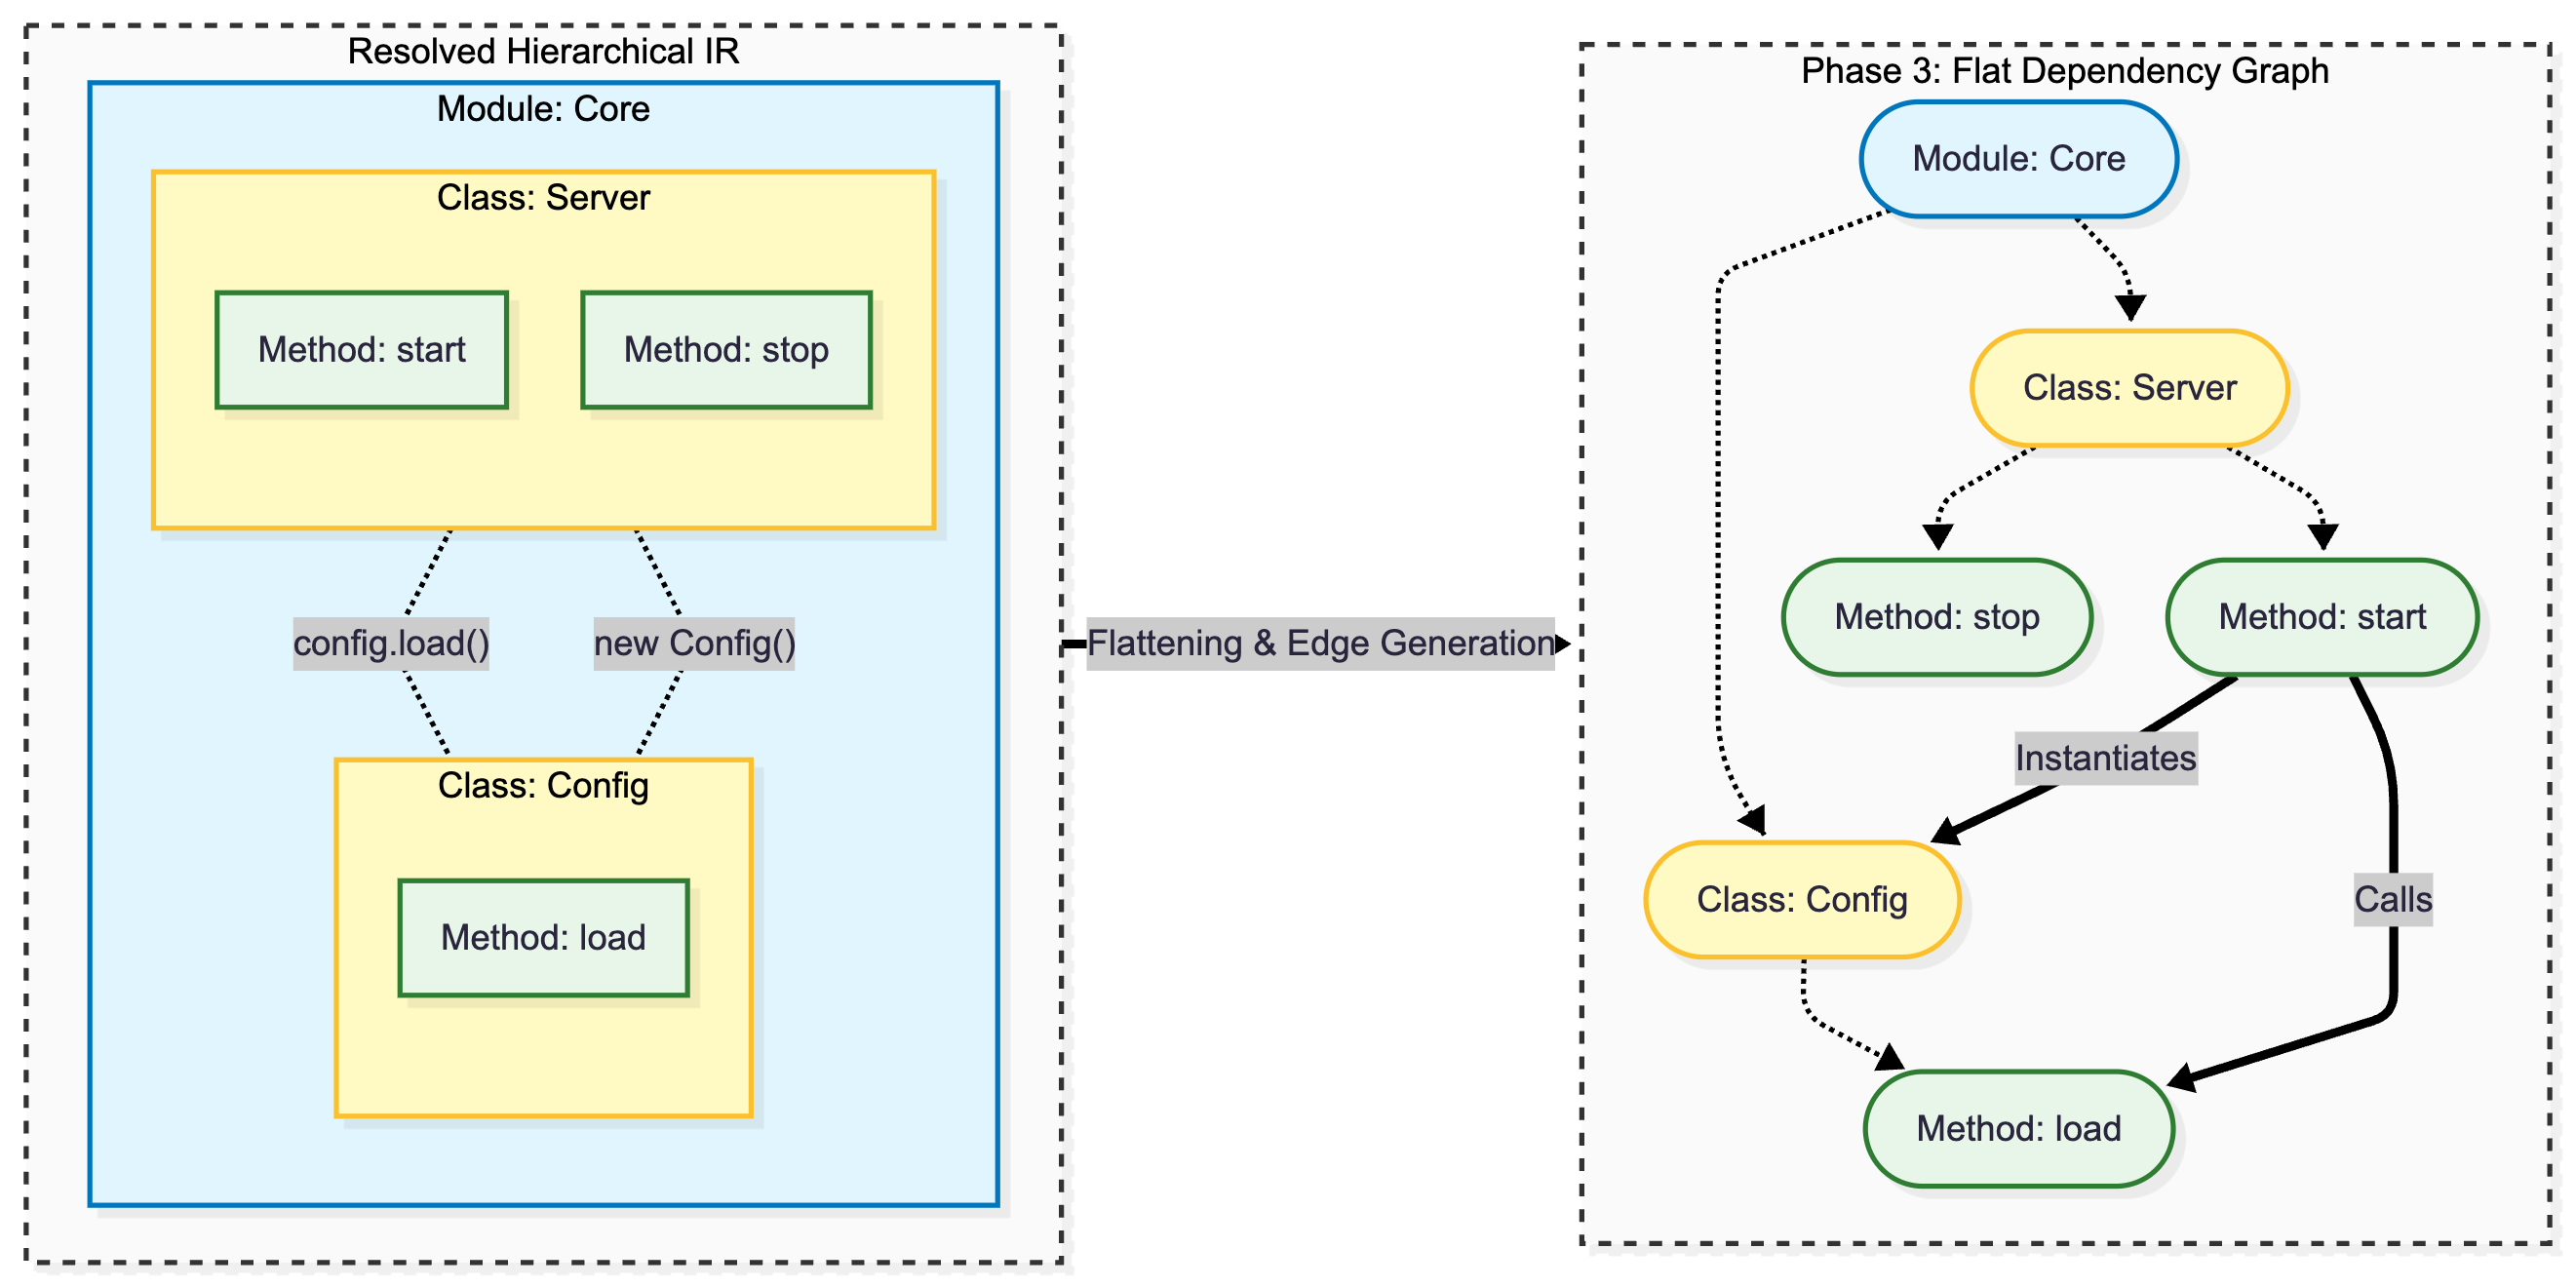
\includegraphics[width=\textwidth]{images/formal_ir/graph_flattening_process.png}
  \caption{Visual representation of the Component Tree flattening
    process, where nested elements are promoted to top-level graph
    nodes and hierarchical containment is converted to directed structural edges
  (\texttt{ModuleContainment} and \texttt{NestedIn}).}
  \label{fig:graph_flattening}
\end{figure}
